\documentclass[10pt]{article}
\usepackage{pgf,tikz,pgfplots}
\pgfplotsset{compat=1.15}
\usepackage{mathrsfs}
\usetikzlibrary{arrows}
\pagestyle{empty}
\begin{document}
\definecolor{rvwvcq}{rgb}{0.08235294117647059,0.396078431372549,0.7529411764705882}
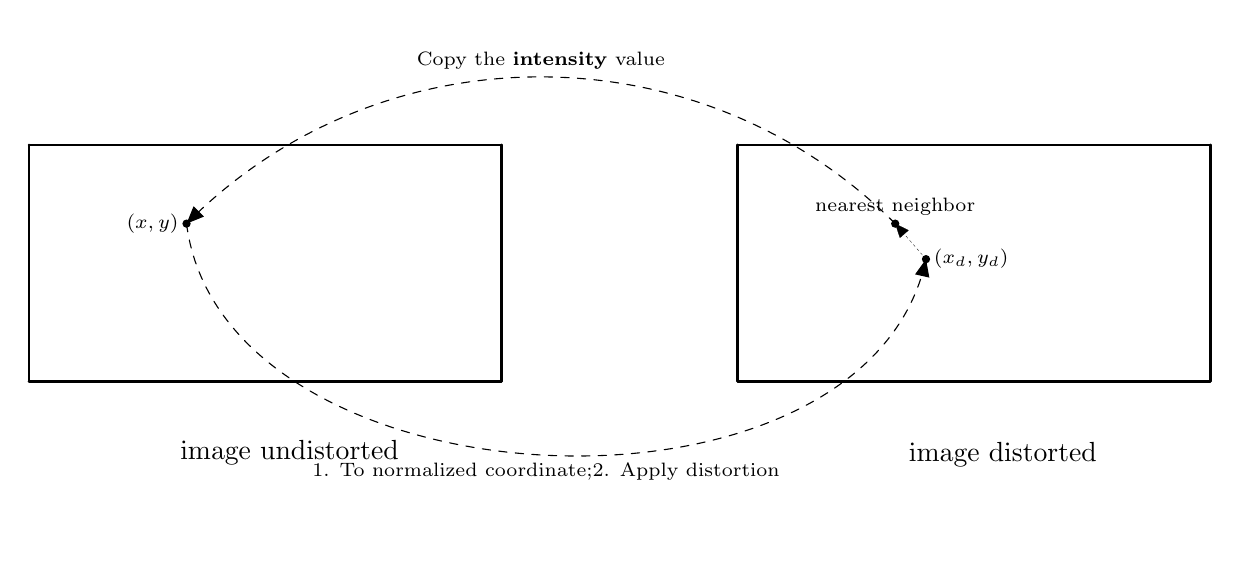
\begin{tikzpicture}[line cap=round,line join=round,>=triangle 45,x=1cm,y=1cm]
%\clip(-16.603845000318117,-3.7496660030175057) rectangle (22.761462065313584,6.118325057125529);
\draw [line width=1pt] (-7,3)-- (-7,0);
\draw [line width=1pt] (-1,0)-- (-1,3);
\draw [line width=1pt] (-7,3)-- (-1,3);
\draw [line width=1pt] (-7,0)-- (-1,0);
\draw [line width=1pt] (2,3)-- (2,0);
\draw [line width=1pt] (2,0)-- (8,0);
\draw [line width=1pt] (8,3)-- (8,0);
\draw [line width=1pt] (8,3)-- (2,3);
\draw (-5.203243083907896,-0.629274066577513) node[anchor=north west] {image undistorted};
\draw (4.050160265286048,-0.6491491744529269) node[anchor=north west] {image distorted};

\begin{scriptsize}
\draw[fill=black, draw = none] (-5,2) circle (1.5pt) node[above,left] {$(x,y)$};
\draw[fill=black, draw = none] (4.391239669421487,1.5490082644628136) circle (1.5pt) node[right] {$(x_d,y_d)$};
\draw[fill=black, draw = none] (4,2) circle (1.5pt) node[above] {nearest neighbor};


	\coordinate (A1) at  (-5,2);
	\coordinate (A2) at  (4.391239669421487,1.5490082644628136);
	\coordinate (A3) at  (4,2);

\draw [->, line width=0.1pt,dash pattern=on 1pt off 1pt] (A2)-- (A3);
	\draw[->, dashed] (A1) to[bend left=-80] node[below,rotate=0] {1. To normalized coordinate; \newline 2. Apply distortion} (A2);
	
	\draw[->, dashed] (A3) to[bend right=45] node[above,rotate=0] {Copy the \textbf{intensity} value} (A1);


%\draw [fill=rvwvcq] (-5,2) circle (1.0pt) node {(x,y)};
%\draw[color=rvwvcq] (-4.385262677349315,2.1780849208247095) node ;
%\draw [fill=rvwvcq] (4.391239669421487,1.5490082644628136) circle (1.0pt);
%\draw[color=rvwvcq] (5.149321436599141,1.7507701015033097) node {$(x_d,y_d)$};
%\draw [fill=rvwvcq] (4,2) circle (1.5pt);
\end{scriptsize}
\end{tikzpicture}
\end{document}